
%(BEGIN_QUESTION)
% Copyright 2011, Tony R. Kuphaldt, released under the Creative Commons Attribution License (v 1.0)
% This means you may do almost anything with this work of mine, so long as you give me proper credit

{\it Hydrocracking} is a petroleum refining process whereby heavy oils are converted into lighter oils for use as jet fuel and feedstock for gasoline production.  In a hydrocracker reactor, heavy oils such as octane (C$_{8}$H$_{18}$) are mixed with hydrogen gas (H$_{2}$) at high temperatures and pressures to form lighter compounds such as propane (C$_{3}$H$_{8}$) and pentane (C$_{5}$H$_{12}$):

$$\includegraphics[width=15.5cm]{i03418x01.eps}$$

Expressed in formula form, this reaction is as follows:

$$\hbox{C}_8 \hbox{H}_{18} + \hbox{H}_2 \to \hbox{C}_3 \hbox{H}_{8} + \hbox{C}_5 \hbox{H}_{12}$$

\vskip 10pt

Overall, such reactions are exothermic.  However, not every {\it portion} of the reaction is exothermic.  Identify the endothermic and exothermic processes at work in a typical hydrocracking reaction, and comment on their relative energies given the knowledge that the overall reaction is exothermic.

\vskip 30pt

Given the exothermic nature of hydrocracking reactions, some form of cooling is needed to prevent a ``runaway'' condition.  In modern hydrocracker reactors, excess hydrogen gas is injected at the catalyst beds to ``quench'' the reaction and thereby control temperature.  Based on what you know about hydrogen, explain why it is an effective coolant for this process.

\vfil 

\underbar{file i03418}
\eject
%(END_QUESTION)





%(BEGIN_ANSWER)

This is a graded question -- no answers or hints given!
 
%(END_ANSWER)





%(BEGIN_NOTES)

Breaking the C-C bond in the original octane molecule is an endothermic process, as is the breaking of the H-H bond in the H$_{2}$ molecule.  However, the formation of new C-H bonds is exothermic, and we may deduce from the overall exothermic classification of this reaction that the amount of heat liberated by the formation of new C-H bonds exceeds the energy needed to break the old C-C and H-H bonds.

\vskip 10pt

Hydrogen gas has an extremely high specific heat value, making it an excellent coolant for this process.

%INDEX% Chemistry, basic: molecular bonds and energy exchange

%(END_NOTES)


